% report_31_01_2018.tex
% Omkar H. Ramachandran
% omkar.ramachandran@colorado.edu
%
% Documentation for hemispheric dependence in the Fermi Pass 8 data
%

\documentclass[english]{article}
\usepackage[T1]{fontenc}
\usepackage[latin9]{inputenc}
\usepackage{geometry}
\geometry{verbose,tmargin=1.5in,bmargin=1.5in,lmargin=1.5in,rmargin=1.5in}
\usepackage{babel}
\newcommand{\GeV}{\,{\rm GeV}}
\usepackage{graphicx}
\graphicspath{{./plots/}}
\usepackage{listings}

\lstdefinestyle{custompy}{
  belowcaptionskip=1\baselineskip,
  breaklines=true,
  frame=L,
  xleftmargin=\parindent,
  language=Python,
  showstringspaces=false,
  basicstyle=\footnotesize\ttfamily,
  keywordstyle=\bfseries\color{green},
  commentstyle=\itshape\color{red},
  identifierstyle=\color{black},
  stringstyle=\color{blue},
}

\lstset{escapechar=@,style=custompy}


\begin{document}
\title{Hemispheric dependence of the pseudoscalar $Q$ in Pass 8 of the Fermi LAT data}
\author{Omkar H. Ramachandran}

\maketitle

\begin{abstract}
A recent study by Tashiro et al. (2015) proposed a mechanism through which the 
helicity of an extragalactc magnetic field could be estimated by measuring
a CP-odd pseudoscalar $Q$.
A significant observation in their study was the apparent dependence of
this pseudoscalar on the hemisphere where it is measured. 
In this study, we extend the original analysis using 100 weeks of data from 
Pass 8 of the Fermi Large Area Telescope (LAT) to better understand this 
dependence.
\end{abstract}

\section{Method and Setup}
\subsection{Setting up a Monte-Carlo simulation}
If there was no intervening magnetic field between source and detector, the
probability that a photon hits any point on the sphere is identical to the
corresponding probability at any other point.
Therefore, it is possible to model this by setting up a monte-carlo simulation
such that $\cos \theta$ and $\phi$ are uniformly distributed over $[-1,1]$ and
$[0,2\pi]$ respectively.
We further refined this model by taking into account the exposure time at each
latitude and longitude.
The Fermi LAT data comes with a series of spacecraft files that list the time
spent by the satellite at varius positions in the sky.
Using this data -- via the 'gtltcube' tool provided by the 
'sciencetools' package -- we generate an exposure map that determines
the relative likelihood of detecting a photon at a given $l$ and $b$.
Figure \ref{fig:montecarlo} shows the measured value of $Q$ for a montecarlo
simulation with 10551 photons in the low energy bin, 1348 photons in the 
intermediate bin and 550 in the highest energy bin repeated over 20 iterations.
Already, we see that the montecarlo predicts the sign of $Q$ to be zero
within error bars.
However, the most extreme realization out of the twenty -- decided by selecting
for the largest RMS distance from the mean -- can be more than a standard
deviation away from the mean, especially at large $R$
\begin{figure}
	\centering
	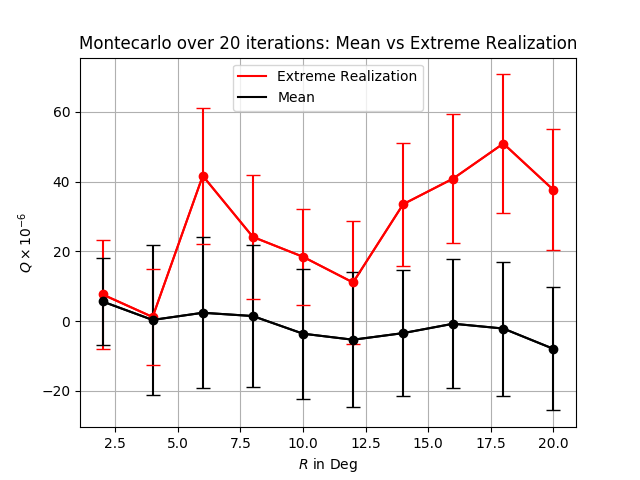
\includegraphics[scale=0.5]{montecarlo_meanvextreme.png}
	\caption{Monte-Carlo simulation of the pseudoscalar $Q$ if there were no
	intervening field. It is evident from the plot that the mean value of $Q$
	always zero within the error-bars}
	\label{fig:montecarlo}
\end{figure}

\section{Calculating $Q$ from the Fermi Data}
\begin{figure}
	\centering
	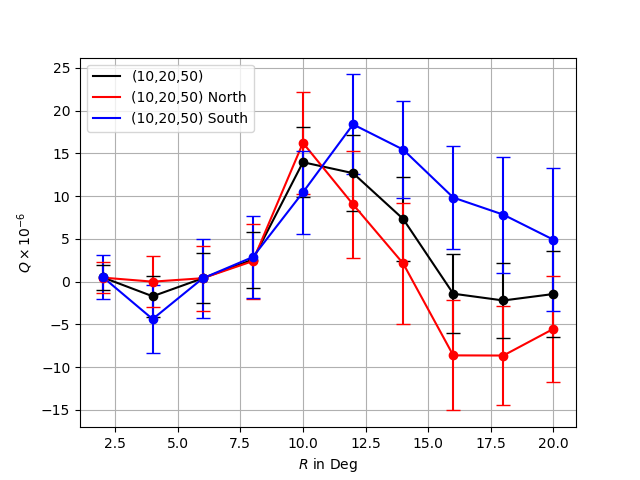
\includegraphics[scale=0.5]{Qhemisphere_wk_100_400_10_20_50_scrubbed.png}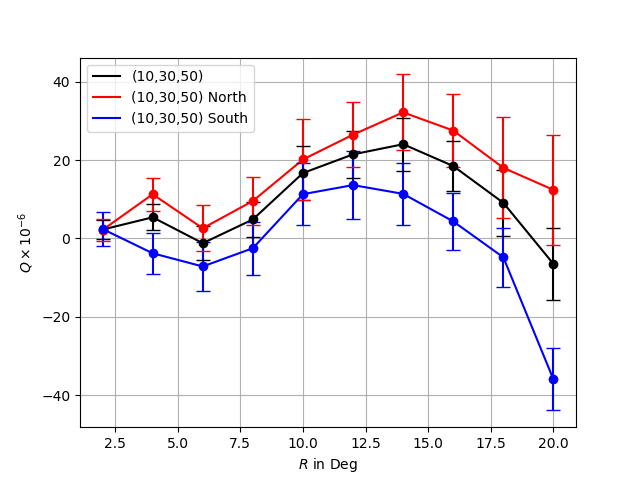
\includegraphics[scale=0.5]{Qhemisphere_wk_100_400_10_30_50_scrubbed.png}

	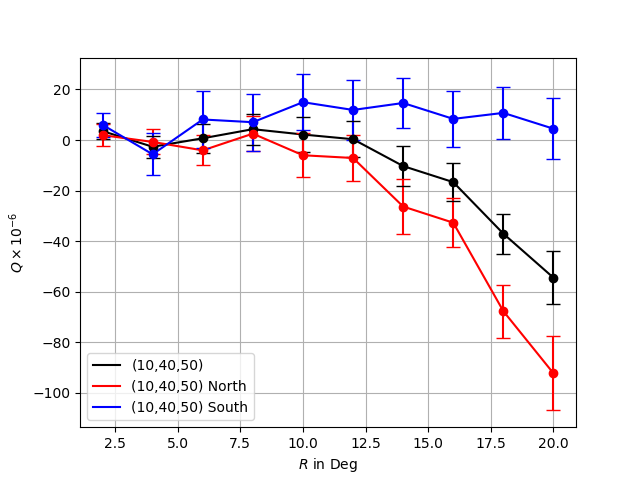
\includegraphics[scale=0.5]{Qhemisphere_wk_100_400_10_40_50_scrubbed.png}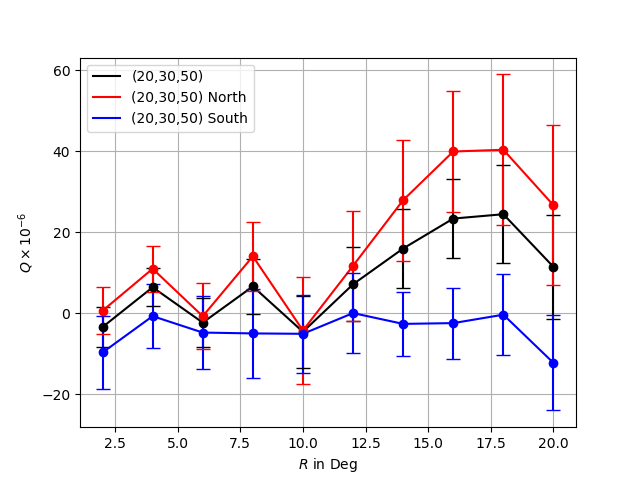
\includegraphics[scale=0.5]{Qhemisphere_wk_100_400_20_30_50_scrubbed.png}
	
	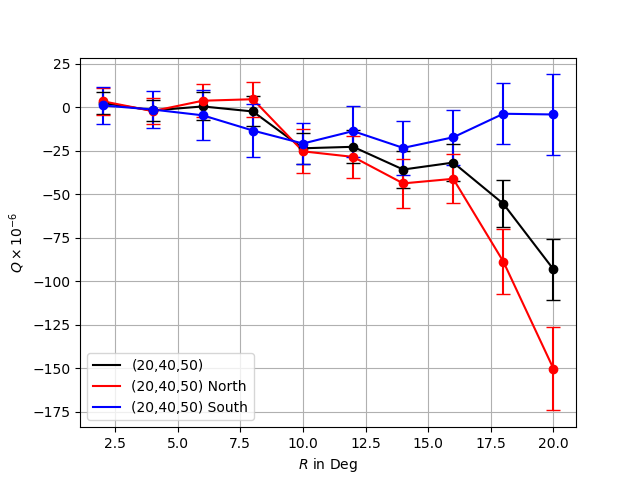
\includegraphics[scale=0.5]{Qhemisphere_wk_100_400_20_40_50_scrubbed.png}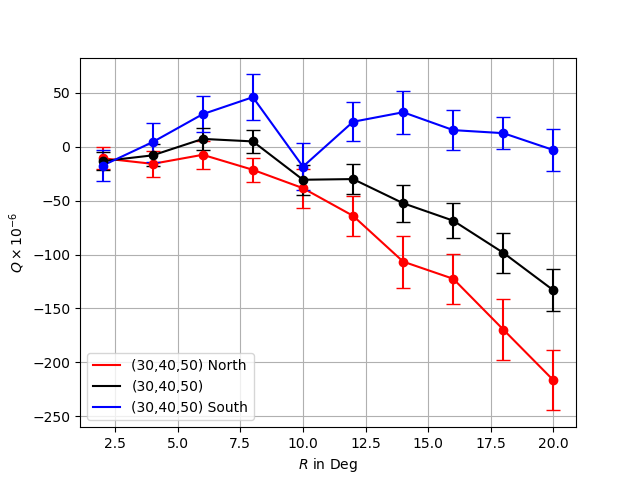
\includegraphics[scale=0.5]{Qhemisphere_wk_100_400_30_40_50_scrubbed.png}
	\caption{(Clockwise from top) Plot of computed value of $Q$ as a function
	of $R$ for (a) 10,20,50 (b) 10,30,50 (c) 20,30,50 (d) 30,40,50 (e) 20,40,50
	and (f) 10,40,50}
	\label{fig:hemisphere}
\end{figure}

\subsection{Setup}
In all, the setup used in the following section closely resembled the setup
used by Tashiro et al. (2015). In particular,
\begin{itemize}
\item For measuring $Q$, we used $404$ weeks of data from Pass 8 of the Fermi 
	LAT, specifically, from weeks 100 through 504.
\item To avoid contamination from the galactic disk, only photons present in
	the region on the sky described by $b > 70^{\circ}$ was considered.
\item To avoid contamination from cosmic ray scattering in the upper
	atmosphere, photons arriving at Zenith angles greater than $100^{\circ}$ 
	were discarded.
\item Finally, the selected data with these characteristics was filtered so as
	to only use photons that were marked as 'clean' using the 'gtmktime' command
	in the sciencetools package. The spacecraft's rocking angle at the time of 
	event detection was also constrained to a maximum $52^{\circ}$.
\end{itemize}

\subsection{$l_{E_3} > 70^{\circ}$}

\subsubsection{$E_1 = 10 \GeV$}
Looking at Figure \ref{fig:hemisphere}, we observe that for two of the three
energy combinations (10,20,50 and 10,30,50), the $Q$ vs $R$ curves for the 
northern and southern hemispheres track each other. 
For (10,40,50) however, we see sharp hemispheric dependence with a strong negative
trend for the curve in the northern hemisphere that isn't seen in the 
corresponding curve for the southern hemisphere.
As will be demonstrated in the remaining two sections, this dependence seems
to appear only in combinations that include the $40$ to $50$ $\GeV$ bin.

\subsubsection{$E_1 = 20 \GeV$}
Once again, we observe that only the bin combination with $40$ to $50$ $\GeV$
(Figure \ref{fig:hemisphere}(e)) shows sharp hemispheric dependence. 
For the remaining combinations, the overall value of $Q$ at $R=20$ is zero within
errorbars.

\subsubsection{$E_1 = 30 \GeV$}
When the lowest energy bin is set at $30 \GeV$, there is exactly one combination
that is possible: 30,40,50 (Figure \ref{fig:hemisphere}(d)).
Here, we observe that the curve is similar to 40,50 combination in the previous 
sections, with the northern curve being significantly more negative than the
southern curve.


\begin{figure}
	\centering
	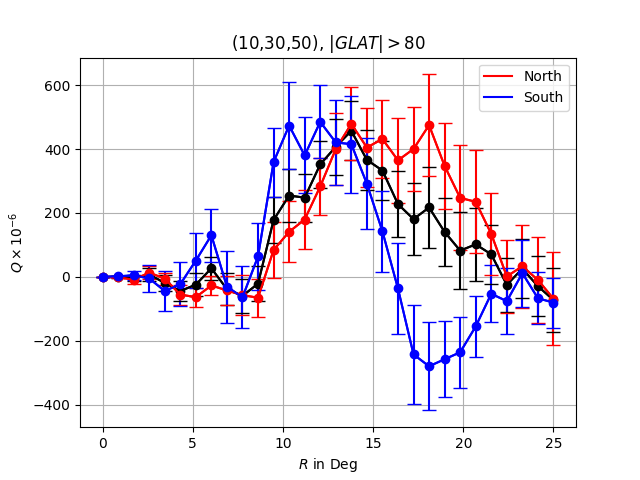
\includegraphics[scale=0.5]{10_30_50_full.png}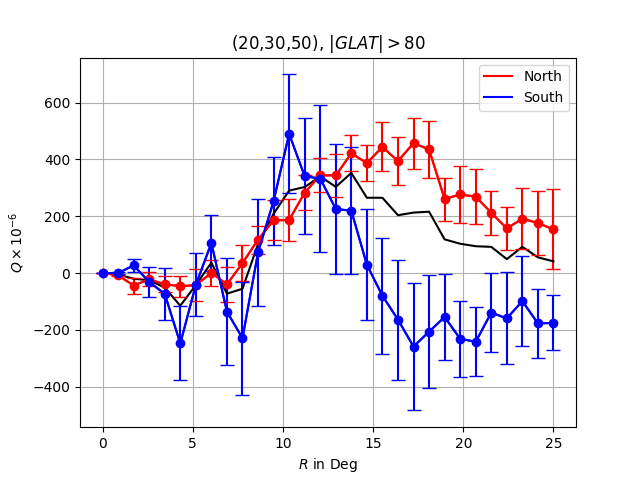
\includegraphics[scale=0.5]{20_30_50_full.png}
	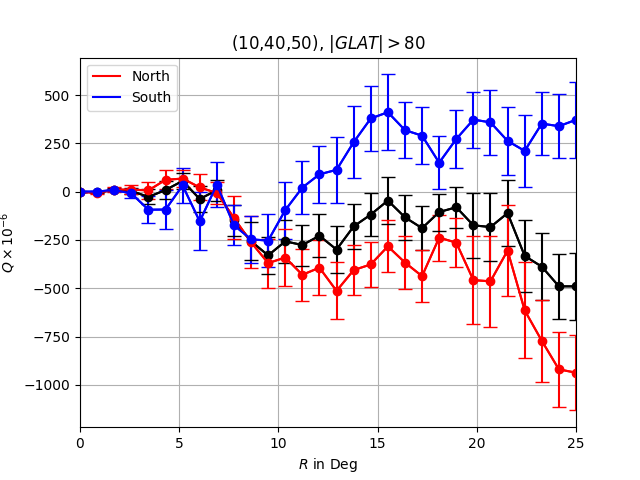
\includegraphics[scale=0.5]{10_40_50_full.png}
	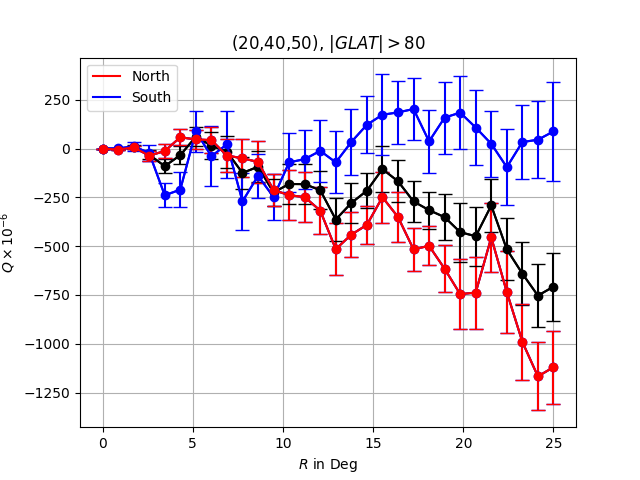
\includegraphics[scale=0.5]{20_40_50_full.png}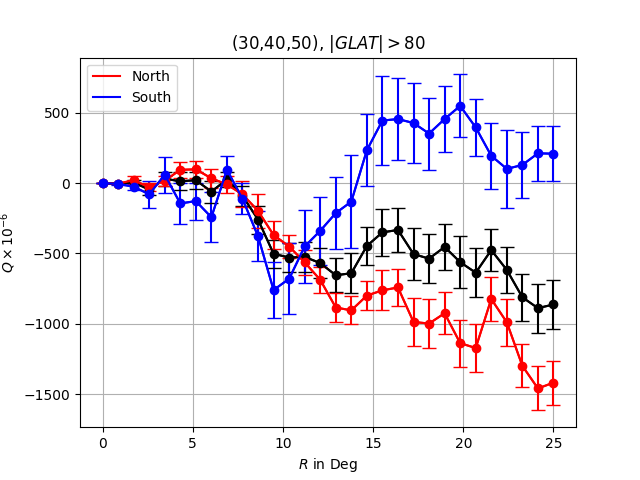
\includegraphics[scale=0.5]{30_40_50_full.png}

	\caption{Plots of $Q$ vs the patch radius $R$ around each $E_3$
	point for (top) $E_2 = 30\ \GeV$ and (middle and bottom) 
	$E_2=40\ \GeV$}
	\label{fig:hemisphere_lg80}
\end{figure}



\begin{figure}
	\centering
	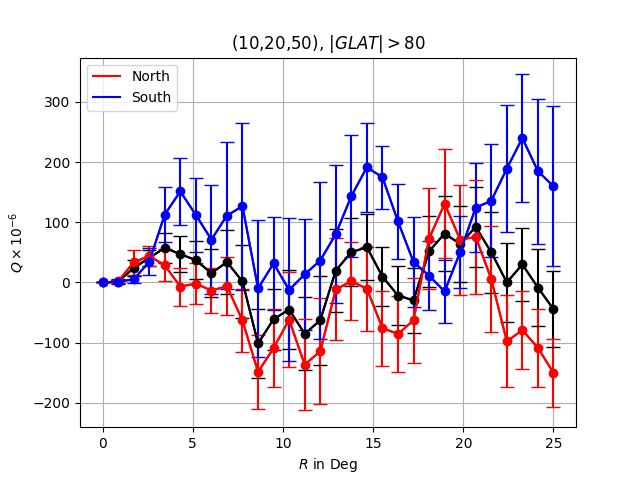
\includegraphics[scale=0.5]{10_20_50_full.png}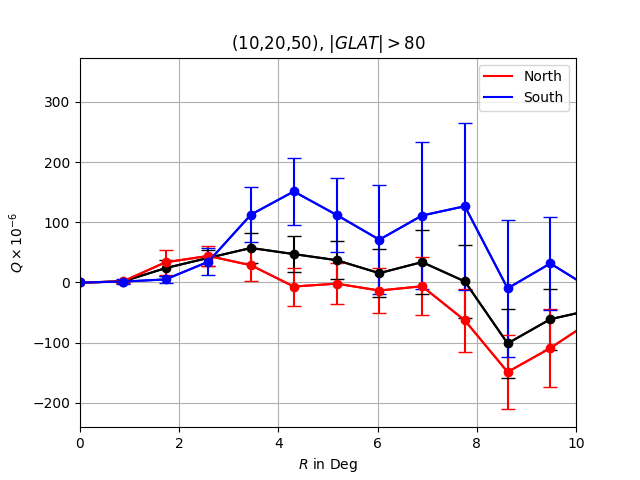
\includegraphics[scale=0.5]{10_20_50_upto_10.png}
	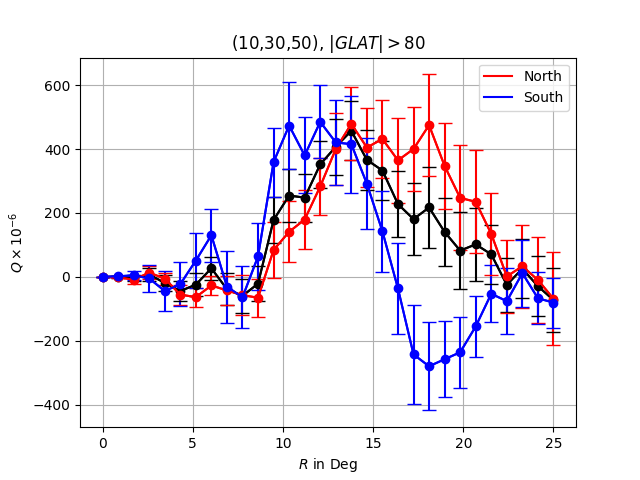
\includegraphics[scale=0.5]{10_30_50_full.png}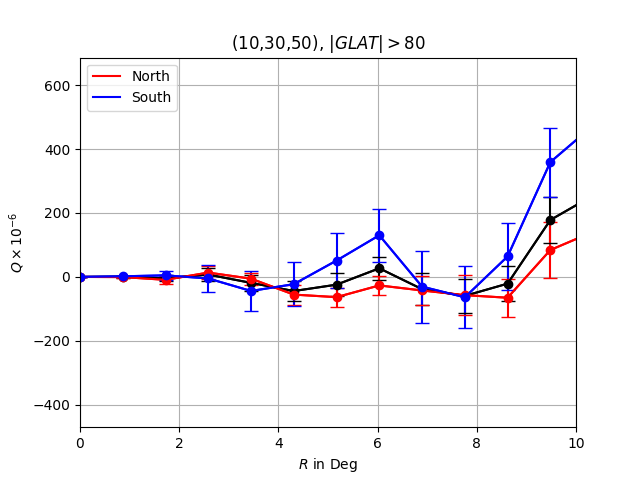
\includegraphics[scale=0.5]{10_30_50_upto_10.png}
	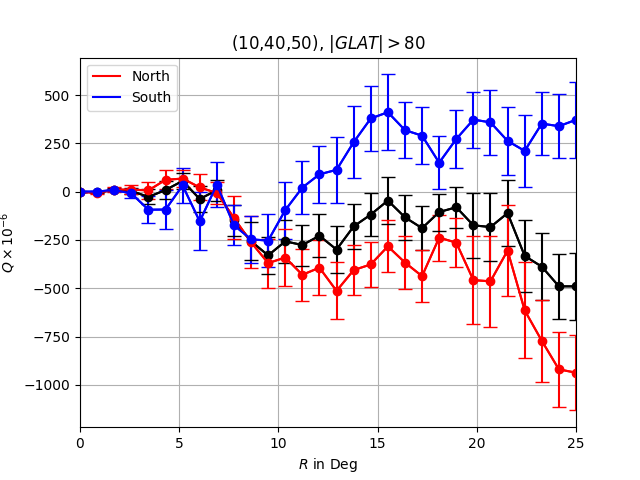
\includegraphics[scale=0.5]{10_40_50_full.png}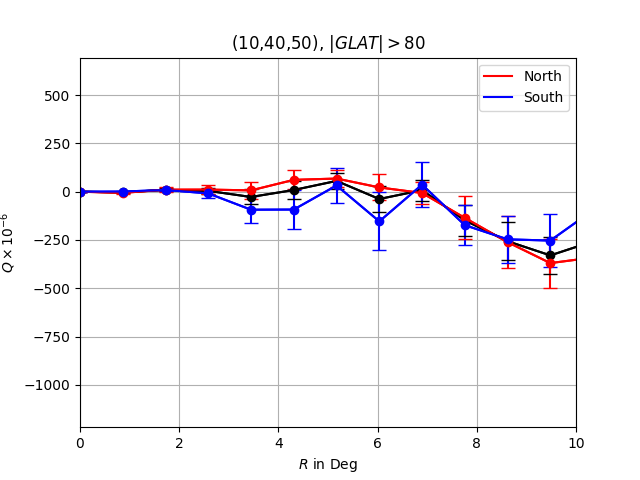
\includegraphics[scale=0.5]{10_40_50_upto_10.png}

	\caption{(Top to bottom) Plots of $Q$ vs the patch radius $R$ around each $E_3$
	point for (left) $R\in[0^{\circ},25^{\circ}]$ and (right) 
	$R\in[0^{\circ},10^{\circ}]$, $E_{1} = 10\ \GeV$ and $l>80^{\circ}$}
	\label{fig:hemisphere_lg80}
\end{figure}



\subsection{$l_{E_3} > 80^{\circ}$}
When we restrict our patches to points in the $E_{3}$ energy bin that are higher
than $|l| > 80^{\circ}$.
In this scenario, we see that there are two distinct regimes for all but one of
the energy bin combinations (10,20,50) Figure \ref{fig:hemisphere_lg80}.1.
Specifically, we observe that when we consider $R\leq10^{\circ}$ -- thus 
purely constraining ourselves to latitudes where the galactic disk is
expected to have minimal impact --, there is no hemispheric dependance.
As in section 2.1, we observe that the intermediate bin is a very good
predictor of the $Q$ vs $R$ trend (Figure \ref{hemisphere_lg80}).
We also find that $Q$ is weakly positive or zero under these circumstances
for $E_{2}\in{20,30}\ \GeV$ and is strongly negative only for 
$E_2=40\ \GeV$.
This result further evidences the possibility that the hemispheric dependence
seen at high $R$ for the $l_{E_3}\geq70^{\circ}$ case is simply a case
of interference from the galactic disk, but we would need a full model of 
the galactic disk added into the Monte-Carlo simulation to confirm this
possibility.

\section{Discussion}
In each of the three cases discussed in the previous section, we observe that
the strong negative trend for $Q$ as well as the sharp hemispheric dependence
seems to appear only in the ($E_1$,40,50) bin. 
This might point to contamination in the $40$ to $50$ $\GeV$ bin that hasn't 
been accounted for in this setup, or it might point to some interesting 
physics.
Having said this, in each of the cases presented above, we find that the 
deviation between the measured overall value and the northern and southern
curve is at least $\sigma$ - with the exception of Figure 2(a).
Interestingly, the overall value of $Q$ is sharply negative only when we 
include the $40-50\ \GeV$ bin.
In all other cases, $Q$ is either weakly positive, or zero within error bounds.

\end{document}
